\documentclass{article}
\usepackage{titlesec}
\usepackage[dotinlabels]{titletoc}
\usepackage[utf8]{inputenc}
\usepackage[russian]{babel}
\usepackage[a4paper, left=1.5cm, right=1.5cm, top=1cm, bottom=1cm]{geometry}
\usepackage[unicode, pdftex]{hyperref}
\setlength\parindent{0pt}
\pagenumbering{gobble}
\usepackage{caption} 
\captionsetup[table]{skip=5pt}
\usepackage{graphicx}
\usepackage{float}

\begin{document}

\begin{minipage}{0.62\textwidth}
    \begin{center}
        Санкт-Петербургский национальный исследовательский университет \\
        информационных технологий, механики и оптики \\
        УЧЕБНЫЙ ЦЕНТР ОБЩЕЙ ФИЗИКИ ФТФ
    \end{center}
\end{minipage}
\hfill
\begin{minipage}{0.38\textwidth}
    \centering
    \begin{figure}[H]
    
\includegraphics[width=\textwidth]{logo.png}
    \end{figure}
\end{minipage}

\rule{\textwidth}{1pt} \\

\begin{minipage}{0.16\textwidth}
        Группа \hrulefill\\
        Студент \hrulefill\\
        Преподаватель \hrulefill
\end{minipage}%
\begin{minipage}{0.25\textwidth}
        K3222\hrulefill\\
        Бевз Т.А.\hrulefill\\
        Соломонов А.И.\hrulefill
\end{minipage}
\hfill
\begin{minipage}{0.47\textwidth}
        К работе допущен \hrulefill\\
        Работа выполнена \hrulefill\\
        Отчёт принят \hrulefill
\end{minipage}
\begin{center}
    \textbf{\huge Рабочий протокол и отчет по \\
    лабораторной работе № 5.01}
\end{center}
\begin{minipage}{1\textwidth}
        \hrulefill\\
        \Large\textbf{Измерение температуры и интегрального коэффициента излучения тела методом спектральных отношений}\hrulefill
\end{minipage}
\section{Цель работы}
\begin{enumerate}
     Определение значения интегрального коэффициента излучения $A_T$ источника, исследование зависимость $A_T$ от температуры.
\end{enumerate}

\section{Задачи, решаемые при выполнении работы}
\begin{enumerate}
    \item Измерение относительной интенсивности фототока для двух волн при различных напряжениях накала.
    \item Вычисление температуры источника при различных значениях напряжения источника.
    \item Вычисление мощности на спирали при различных температурах.
    \item Построение графика зависимости мощности от температуры, определение мощности при температуре 2000К.
    \item Вычисление значений интегрального коэффициента излучения для различных температур.
    \item Построение графика зависимости интегрального коэффициента излучения от температуры.
\end{enumerate}

\section{Объект исследования}
Источник излучения.
\section{Метод экспериментального исследования}
Физический эксперимент.
\section{Рабочие формулы и исходные данные}
\begin{equation}
 T=\frac{L}{ln\frac{J_1}{J_2}-Z_0} - \textit{Температура источника накала.}
 \label{eq:ref1}
\end{equation}
Где $L=C_2(\frac{1}{\lambda_2}-\frac{1}{\lambda_1})$
Где $Z_0 = 1.784$; $C_2=1.439\cdot 10^{-2}$
\begin{equation}
 P_{\textit{ист}}=IU - \textit{Мощность источника.}
 \label{eq:ref2}
\end{equation}
\begin{equation}
 A_T= A_{2000}\cdot K \cdot \frac{P_{\textit{ист}}}{T^4} - \textit{интегральный коэффициент излучения.}
 \label{eq:ref3}
\end{equation}
Где $A_{2000}=0.249$; $K=\frac{2000^4}{P_{\textit{ист}2000}}$
\newpage
\section{Измерительные приборы}
\begin{table}[h]
    \centering
    \bgroup
    \def\arraystretch{1.2}
    \begin{tabular}{|c|c|c|c|}
        \hline
        Наименоване & Тип прибора & Используемый диапазон & Погрешность \\
        \hline
        Блок РТИ-1 & Цифровой & $5-11$ В & $0.01$ В \\
        \hline
    \end{tabular}
    \egroup
    \caption{Измерительные приборы} 
\end{table}
\section{Ход работы}
\begin{itemize}
  \item Для обработки результатов лабораторной работы было необходимо снять показания с цифрового индикатора измерителя относительной интенсивности теплового излучения ($\frac{J_1}{J_0}$ и $\frac{J_2}{J_0}$), амперметра ($I$) и вольтметра ($U$). Результаты представлены в таблице №2.
  \item Далее для каждого измерения были вычислены $\frac{J_1}{J_2}$, $T$, $P$ и $A_T$. Вычисления представлены в таблице №2.
  \item На основе полученных данных был построен и апроксимирован график зависимости мощности на источнике от температуры накала $ P_{\textit{ист}}(T) $, также было определено значение мощности при температуре 2000 K $P_{\textit{ист}2000} = 2.213$ Вт. График представлен на рисунке №1. И график зависимости интегрального коэффициента излучения от температуры накала $ A_{T}(T) $. График представлен на рисунке №2.
\end{itemize}
\section{Результаты прямых измерений и их обработки}
\begin{table}[h]
    \centering
    \bgroup
    \def\arraystretch{1.4}
    \begin{tabular}{|c|c|c|c|c|c|c|c|c|}
        \hline
        № & $I$, мA & $U$, В & $\frac{J_1}{J_0}$ & $\frac{J_2}{J_0}$ & $\frac{J_1}{J_2}$ & $T$, K & $P$, Вт & $A_{T}$ \\ \hline
        $ 1 $ & $ 197 $ & $ 5.22 $ & $ 0.007 $ & $ 0.075 $ & $ 0.093 $ & $ 1562.8 $ & $ 1.028 $ & $ 0.310 $\\ \hline
        $ 2 $ & $ 203 $ & $ 5.60 $ & $ 0.011 $ & $ 0.101 $ & $ 0.109 $ & $ 1623.1 $ & $ 1.137 $ & $ 0.295 $\\ \hline
        $ 3 $ & $ 209 $ & $ 6.01 $ & $ 0.016 $ & $ 0.133 $ & $ 0.120 $ & $ 1664.5 $ & $ 1.256 $ & $ 0.295 $\\ \hline
        $ 4 $ & $ 216 $ & $ 6.41 $ & $ 0.024 $ & $ 0.172 $ & $ 0.140 $ & $ 1730.3 $ & $ 1.385 $ & $ 0.278 $\\ \hline
        $ 5 $ & $ 222 $ & $ 6.88 $ & $ 0.036 $ & $ 0.225 $ & $ 0.160 $ & $ 1795.8 $ & $ 1.527 $ & $ 0.264 $\\ \hline
        $ 6 $ & $ 228 $ & $ 7.25 $ & $ 0.047 $ & $ 0.272 $ & $ 0.173 $ & $ 1834.8 $ & $ 1.653 $ & $ 0.263 $\\ \hline
        $ 7 $ & $ 233 $ & $ 7.65 $ & $ 0.062 $ & $ 0.327 $ & $ 0.190 $ & $ 1884.2 $ & $ 1.782 $ & $ 0.255 $\\ \hline
        $ 8 $ & $ 239 $ & $ 8.08 $ & $ 0.082 $ & $ 0.394 $ & $ 0.208 $ & $ 1936.6 $ & $ 1.931 $ & $ 0.247 $\\ \hline
        $ 9 $ & $ 245 $ & $ 8.50 $ & $ 0.104 $ & $ 0.465 $ & $ 0.224 $ & $ 1979.0 $ & $ 2.083 $ & $ 0.244 $\\ \hline
        $ 10 $ & $ 251 $ & $ 8.97 $ & $ 0.134 $ & $ 0.553 $ & $ 0.242 $ & $ 2028.6 $ & $ 2.251 $ & $ 0.239 $\\ \hline
        $ 11 $ & $ 256 $ & $ 9.35 $ & $ 0.161 $ & $ 0.626 $ & $ 0.257 $ & $ 2067.0 $ & $ 2.394 $ & $ 0.236 $\\ \hline
        $ 12 $ & $ 261 $ & $ 9.74 $ & $ 0.195 $ & $ 0.712 $ & $ 0.274 $ & $ 2109.2 $ & $ 2.542 $ & $ 0.231 $\\ \hline
        $ 13 $ & $ 267 $ & $ 10.19 $ & $ 0.238 $ & $ 0.815 $ & $ 0.292 $ & $ 2154.1 $ & $ 2.721 $ & $ 0.227 $\\ \hline
        $ 14 $ & $ 272 $ & $ 10.62 $ & $ 0.285 $ & $ 0.918 $ & $ 0.310 $ & $ 2198.8 $ & $ 2.889 $ & $ 0.223 $\\ \hline
        $ 15 $ & $ 275 $ & $ 10.86 $ & $ 0.312 $ & $ 0.975 $ & $ 0.320 $ & $ 2221.5 $ & $ 2.987 $ & $ 0.221 $\\ \hline
    \end{tabular}
    \egroup
    \caption{Результаты прямых измерений и их обработки.} 
\end{table}
\newpage
\section{Графики}
\begin{figure}[h!]
    \begin{center}
    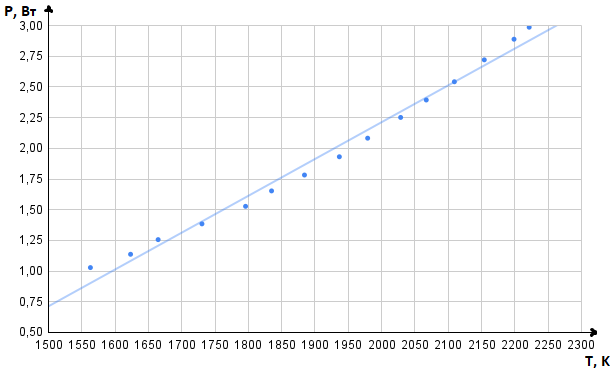
\includegraphics[scale=0.7]{chart1.png}
    \caption{Зависимость мощности на источнике от температуры накала $ P_{\textit{ист}}(T) $}
    \label{fig:graphUfromI}    
    \end{center}
\end{figure}
\begin{figure}[h!]
    \begin{center}
    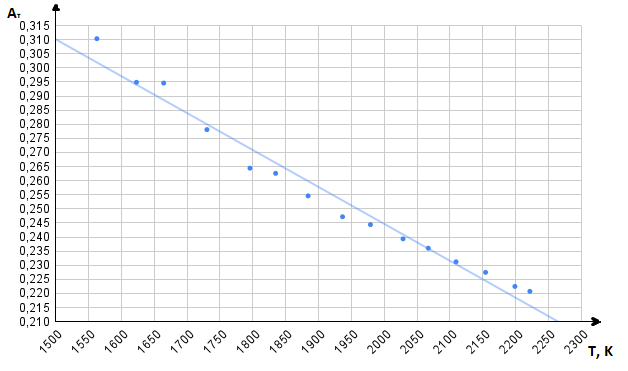
\includegraphics[scale=0.7]{chart2.png}
    \caption{Зависимость интегрального коэффициента излучения от температуры накала $ A_{T}(T) $}
    \label{fig:graphUfromI}    
    \end{center}
\end{figure}
\newpage
\section{Окончательные результаты}
\begin{enumerate}
    \item Мощность на источнике при температуре 2000 К: $P_{2000} = 2.213$ Вт.
\end{enumerate}
\newpage
\section{Вывод}
В ходе работы был изучен метод спектральных отношений. Были определены значения интегрального коэффициента источника в диапазоне температур, была исследована зависимость этого коэффициента от температуры накала и найдена мощность на источнике при температуре 2000К.
\end{document}
